\chapter{Evaluation}

This section presents a comprehensive evaluation of the proposed trading
mechanism, focusing on its performance, scalability, and overall effectiveness
in multi cluster environments. We employ a combination of synthetic and
real-world workloads to simulate various scenarios, alongside an array of rules
and policies to investigate beneficial strategies and the effectiveness of
different workload-strategy combinations.

However, the possible combinations of rules, policies and their respective
configurations is infinite. Our aim in this section is not to exhaust all
possibilities, but to explore the validity of the mechanism under different
constraints. This approach paves the way for users to conduct their experiments
on thier specific workloads to determine the strategies that best fits their
needs.  

All experiments are run on Cloudlab, a scientific infrastructure used by
academics for systems and cloud research [CITE]. We utilize the following
setups to to run the experiments. Each node in the setups simulates one
cluster, with the cluster, trader, and client running on the same machine. 

\begin{enumerate}

  \item \textbf{Setup One:} 3 Cloudlab nodes c6525-100g [CITE] running Linux
    Ubuntu 22.04 in the same Utah datacenter. Cluster sizes are equal having 10
    nodes each with 32 cores and 24GBs of memory.

  \item \textbf{Setup Two:} 3 Cloudlab nodes of type m510, c220g1, c8220 [CITE
    the node configs] running on three distinct datacenters in Utah, Wisconsin,
    and Clemson, and have the same cluster sizes as setup one.

\end{enumerate}

The setups simulate different scenarios where clusters can belong to one
organization, different organizations, and have varying network latency and
bandwidth.  

We derive our results by running a configuration of rules, policies, and
workloads twice, once with and once without the mechanism and compare the
performance difference.

Our methodology for running workloads is as follows, all participating clusters
have the same start and end time for receiving jobs from their respective
clients. After the clients stop sending jobs, the experiment is kept on until
the last job in the slowest cluster finish execution. 

\subsection{Experiment One}

\begin{center}
  \fbox{\parbox{14cm}{
  
    \underline{Configuration:}
    \vspace{.3em}
    \begin{enumerate}
  
      \item \textbf{Setup:} 1 with three cooperative clusters.
  
      \item \textbf{Workload:} Synthetic, all clusters clients' job send rate is
        at 100 per minute derived from a poisson distribution.
      
      \item \textbf{Rules:} Approve trades if average wait time is below 5
        seconds and both memory and core utilization below 0.8
      
      \item \textbf{Policies:} Initiate trades if utilization is above 0.8 or
        average wait time above 60 seconds.
  
    \end{enumerate}
  }}
\end{center}
We will first examine the scenario where all cooperative clusters have high
resource utilization for the entirety of the experiment duration.

%We aim by this experiment to showcase the overhead of the trading mechanism
%where it's likely not beneficial to participate.

\begin{figure}[H]
\centering
\begin{subfigure}{.5\textwidth}
  \centering
  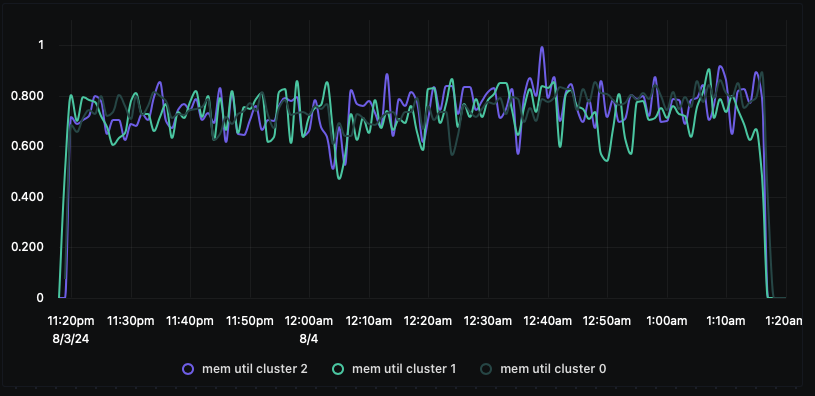
\includegraphics[width=.9\linewidth]{./figures/experiment-one/cooperative-clusters-all-at-100-trading-mem-util.png}
  \caption{cooperative clusters}
  \label{fig:exp1coop}
\end{subfigure}%
\begin{subfigure}{.5\textwidth}
  \centering
  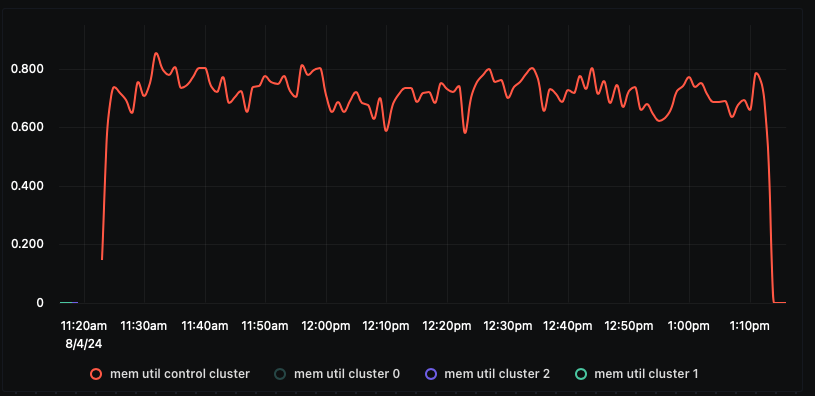
\includegraphics[width=.9\linewidth]{./figures/experiment-one/control-mem-util.png}
  \caption{control cluster}
  \label{fig:exp1control}
\end{subfigure}
\caption{experiment 1, memory utilization}
\label{fig:exp1memutil}
\end{figure}

Figure~\ref{fig:exp1memutil} presents the memory utilization of the cooperative
clusters in \ref{fig:exp1coop} and the same workload run on a cluster without
trading in \ref{fig:exp1control}.
% analysis
We can see that the control cluster have a slightly less utilization averaging
at 70\% whereas cooperative cluster's memory utilization averaged at 75\%. This
5\% difference is due to cooperative clusters slightly benefiting from quick
down time from there peers. We can draw the same conclusion for core
utilization with 65\% and 71\%. However, this led to a 5.45\% increase in
total time to finish all jobs as local resources where occationally lent just
before a spike in jobs, delaying the execution of the local ones. The cluster can't evict external allocations once the
contract is approved.

\subsection{Experiment Two}

\begin{center}
  \fbox{\parbox{14cm}{
  
    \underline{Configuration:}
    \vspace{.3em}
    \begin{enumerate}
  
      \item \textbf{Setup:} 1 with three cooperative clusters.
  
      \item \textbf{Workload:} Synthetic, clusters clients' job send rate is
        100, 50, 10 per minute derived from a poisson distribution.
      
      \item \textbf{Rules:} Approve trades if average wait time is below 5
        seconds and both memory and core utilization below 0.8
      
      \item \textbf{Policies:} Initiate trades if utilization is above 0.8 or
        average wait time above 60 seconds.
  
    \end{enumerate}
  }}
\end{center}

In this experiment, we run trading on a simlar rule and policy configuration as
experiment one, with varying workloads between clusters, detailed in the
configuration box above. 

\begin{figure}[H]
\centering
\begin{subfigure}{.5\textwidth}
  \centering
  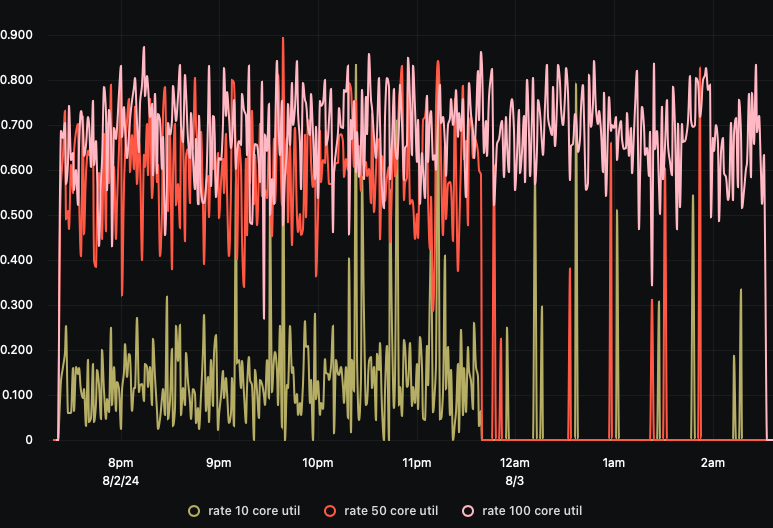
\includegraphics[width=.9\linewidth]{./figures/experiment-two/trading.png}
  \caption{cooperative clusters}
  \label{fig:exp2coop}
\end{subfigure}%
\begin{subfigure}{.5\textwidth}
  \centering
  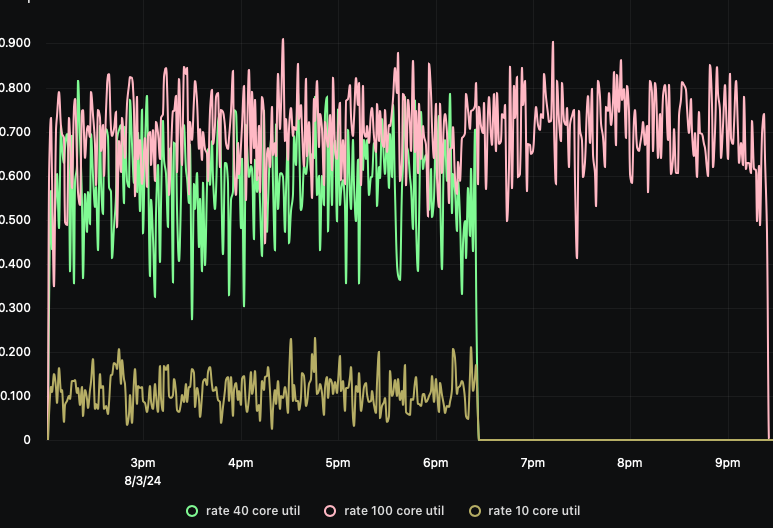
\includegraphics[width=.9\linewidth]{./figures/experiment-two/control.png}
  \caption{control cluster}
  \label{fig:exp2control}
\end{subfigure}
\caption{experiment 2, core utilization}
\label{fig:exp2coreutil}
\end{figure}

Figure~\ref{fig:exp2coreutil} displays the core utilization of the cooperative
clusters in \ref{fig:exp2coop} and the same workload run on a cluster without
trading in \ref{fig:exp2control}.
% analysis
The first evident difference between the two graphs is the spikes seen on the
10 jobs/minute cluster and less apperent the 50 jobs/minute cluster. These
indicate the occurance of trades, benefiting the highly utilized 100
jobs/minute cluster. Trading did not negatively effect the performance of any
of the particpating cluster, and decreased the total time to finish all jobs in the environment by 5.8\%

% the goal is to test different policies and see which ones, coupled with the
% appropriate workload, achieves one of the goals stated in the thesis
% statement.
%\section{Limitations}
%
%- workload overfitting
%https://www.usenix.org/system/files/conference/atc18/atc18-amvrosiadis.pdf
%
%- simulation not actual system
